\section{Motivation}

L’analyse par composantes principales est une technique de réduction de la dimension d’un jeu de données. Elle permet de projeter les données dans un espace restreint tout en conservant le maximum de variance entre les données. 
Les axes utilisés par l’analyse sont appelés composantes principales. Ces composantes principales permettent de transposer les 
données en utilisant les meilleures combinaisons linéaires. Les composantes sont ordonnées de telle sorte qu’elles conservent
 une proportion décroissante de la variance du jeu de données. Les premières composantes sont généralement beaucoup plus 
 informatives que les dernières. Il est ainsi possible de réduire la dimension d’un jeu de données en ne considérant que les premières composantes principales tout en conservant une quantité d’information satisfaisante.\\

Mathématiquement, l’ACP s'exécute en décomposant la matrice de variance-covariance (ou de corrélation) estimée avec le jeu de données en valeurs et vecteurs propres. La matrice de variance-covariance est définie telle que

$$C = Var(X) = \frac{1}{N} \sum_{i = 1}^{N}   \textbf{x}_i\textbf{x}_i^{T} = \frac{1}{N} \sum_{i = 1}^{N}   \textbf{x}_i \cdot \textbf{x}_i$$

La principale limitation de cette méthodologie est qu’elle ne permet pas d’exploiter l’information contenue dans les interactions non linéaires entre les attributs. De plus, les composantes principales sont indépendantes les unes entres elles de telle sorte que l'information non linéaire peut réapparaitre dans les données en conservant un grand nombre de composantes principales. \\

Par exemple, les données dans la figure suivante n'ont aucune de relation linéaire. 

\begin{figure}[H]
	\centering
	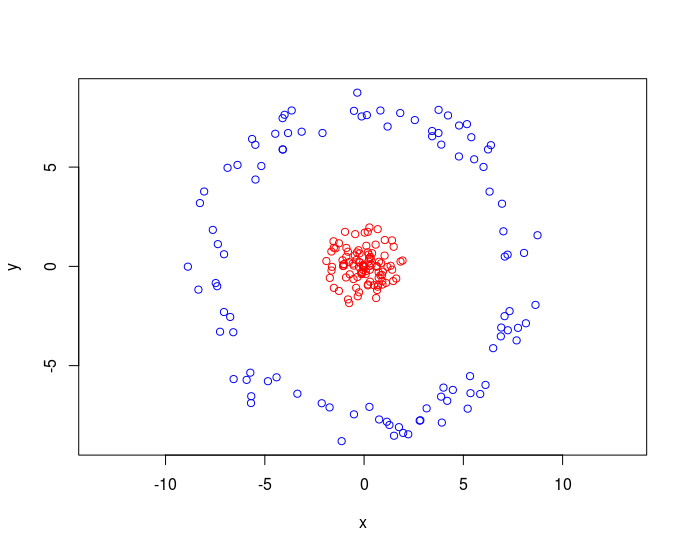
\includegraphics[width=2in]{exemple_1_initial}
\end{figure}

Ensuite, on une transformation non linéaire sur les données et on obtient 

\begin{figure}[H]
	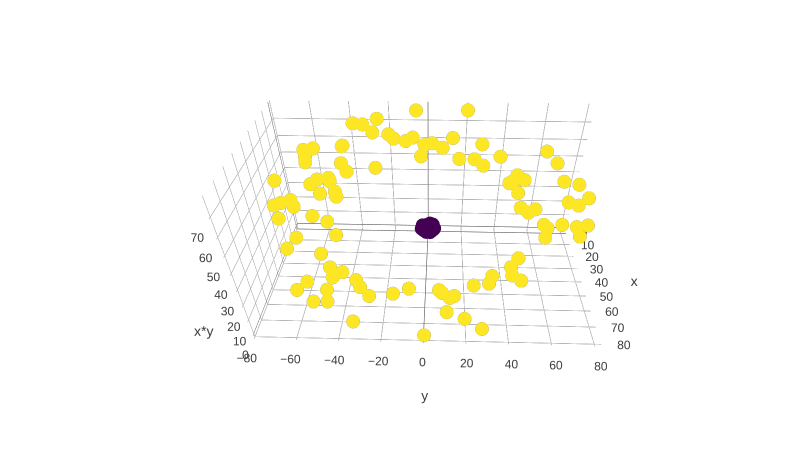
\includegraphics[width=3in]{exemple_1_2d}
\end{figure}

A priori, on ne voit pas l'information additionnelle. Cependant, en appliquant une rotation au graphique, on obtient

\begin{figure}[H]
	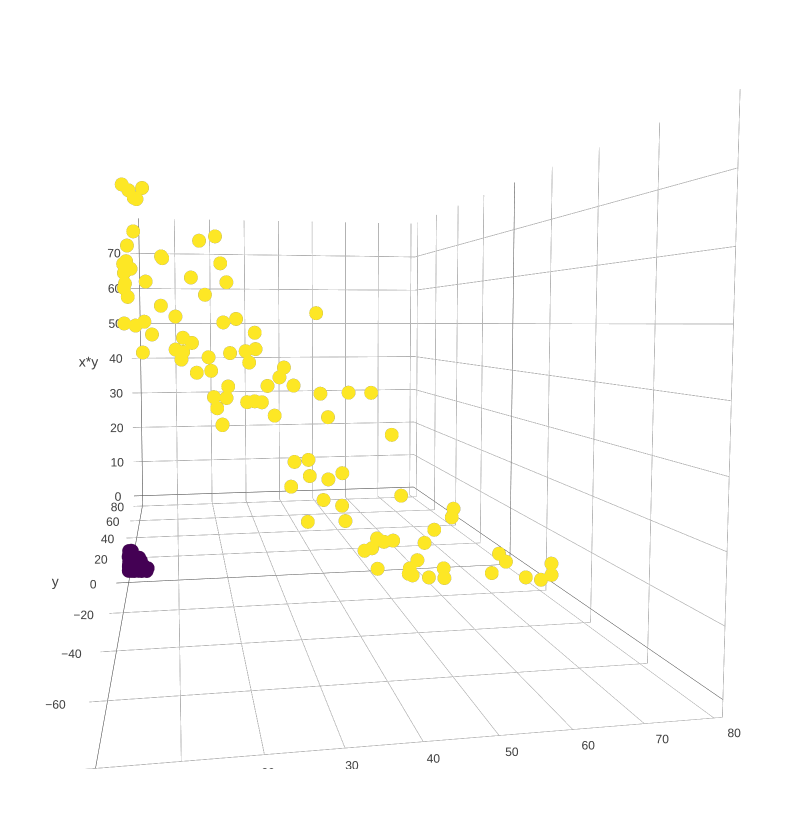
\includegraphics[width=3in]{exemple_1_3d}
\end{figure}

On remarque que ces données peuvent être séparées et interprétées linéairement. Une ACP peut s'appliquer sur ces données transformées et on obtient 

\begin{figure}[H]
	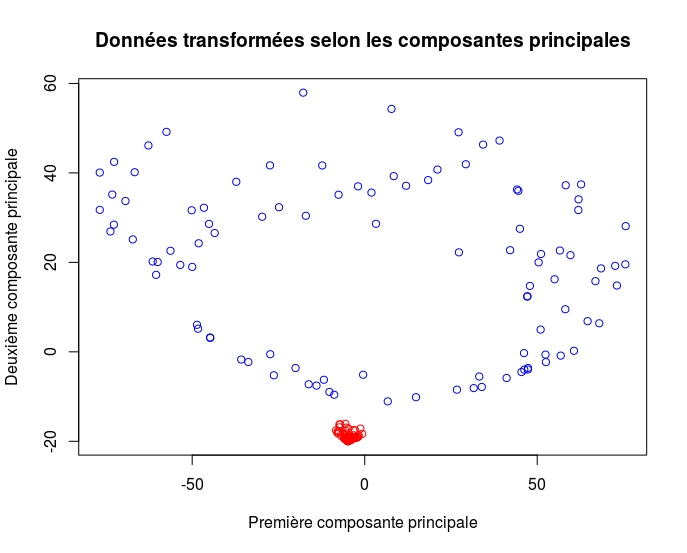
\includegraphics[width=3in]{exemple_1_pca}
\end{figure}

L'idée de l'espace des attributs est de projeter les données originales par une fonction non linéaire vers un nouvel espace qui permet d'interpréter linéairement les relations entre les attributs. Formellement, on a 

\begin{align}\label{eq:featurespace}
\Phi : \mathbb{R}^N &\to \mathcal{F} \nonumber \\
\textbf{x} &\mapsto \Phi(\textbf{x}) 
\end{align}

où les données $\textbf{x}_1, \textbf{x}_2. \dots, \textbf{x}_N \in \mathbb{R}^p$ sont projetées vers un espace d'attributs $\mathcal{F}$ \cite{muller2001introduction}. Souvent, la dimension de $\mathcal{F}$ est beaucoup plus élevée que $p$. L'apprentissage statistique peut maintenant être fait sur les données $$(\Phi(\textbf{x}_1), y_1), (\Phi(\textbf{x}_2), y_2), \dots, (\Phi(\textbf{x}_n), y_n).$$

Afin de motiver cette généralisation du modèle, considérons l'exemple précédent, avec le jeu de données précédent, où
$$\textbf{x}_1, \textbf{x}_2, \dots, \textbf{x}_N = (x_{1,1},x_{1,2}), (x_{2,1}, x_{2,2}), …, (x_{N,1}, x_{N,2})$$

et la transformation utilisée $\Phi(\textbf{x})= (x_1^2 + \sqrt{2} \times x_1\times x_2 + x_2^2)$. La matrice de variance covariance à utiliser pour l’ACP devient
$$\overline{C} = \frac{1}{N} \sum_{i = 1}^{N}   \Phi(\textbf{x}_i) \Phi(\textbf{x}_i)^{T}.$$

Ensuite, on peut reformuler le produit scalaire entre les deux espaces d'attributs comme

\begin{align*}
(\Phi(\textbf{x}_i) \cdot \Phi(\textbf{x}_j)) &= (x_{i, 1}^2 + \sqrt{2} x_{i, 1} x_{i, 2} + x_{i, 2}^2)(x_{j, 1}^2 + \sqrt{2} x_{j, 1} x_{j, 2} + x_{j, 2}^2)^T\\
&= ((x_{i, 1}x_{i, 2})(x_{j, 1}x_{j, 2})^T)^2\\
&= (\textbf{x}_i \cdot \textbf{x}_j)^2.
\end{align*}

En remplaçant avec le résultat précédent, on obtient
$$\overline{C} = \frac{1}{N} \sum_{i = 1}^{N} (\textbf{x}_i \cdot \textbf{x}_j)^2$$ et on doit appliquer une décomposition par valeurs et vecteurs propres sur cette matrice.